\documentclass[12pt]{article}

\usepackage[margin = .8in]{geometry}
\usepackage{amsmath}
\usepackage{graphicx}
\usepackage{multicol, enumerate}

\usepackage{adjustbox}

\usepackage{fancyhdr}
\pagestyle{fancy}

\lhead{Math F113X: Math and Society}
\rhead{Date: \hspace{1in}}

\usepackage{tikz}
\usetikzlibrary{calc,trees,positioning,arrows,fit,shapes,through}
\usetikzlibrary{patterns}

\usetikzlibrary{decorations.markings}
\usetikzlibrary{arrows}

\usepackage{pgfplots}

\usepackage{longtable}
\usepackage{tabularx}

\newcommand{\ds}{\displaystyle}
\newcommand{\ans}[1][1in]{\rule{#1}{.5pt}}

\newcommand{\points}[1]{(#1 points.)}		% Trying to be lazy.

\usepackage{array}
\newcolumntype{L}[1]{>{\raggedright\let\newline\\\arraybackslash\hspace{0pt}}m{#1}}
\newcolumntype{C}[1]{>{\centering\let\newline\\\arraybackslash\hspace{0pt}}m{#1}}
\newcolumntype{R}[1]{>{\raggedleft\let\newline\\\arraybackslash\hspace{0pt}}m{#1}}
\newcommand{\red}[1]{\textcolor{red}{#1}}

\newcommand{\be}{\begin{enumerate}}
\newcommand{\ee}{\end{enumerate}}

%\topmargin -1in
%\textheight 9.5in
%\oddsidemargin -0.3in
%\evensidemargin \oddsidemargin
%\pagestyle{empty}
%%\marginparwidth 0.5in
%\textwidth 7in
%\parindent 0in

%--------------------------------------------------------------------------------------------------------------------------------------------------------------------------
%						Document
%--------------------------------------------------------------------------------------------------------------------------------------------------------------------------


\begin{document}
%\pagestyle{fancy}
\begin{center}
{\Large  Worksheet 11 (Graph Theory 3): Dijkstra's Algorithm}
\end{center}



%\noindent \textbf{Group Names:} \hrulefill \\
%-------------------------------------------------------------------------------------------------------------
%						Assignment
%-----------------------------------------------------------------------------------------------------
\begin{enumerate}
\item Use Dijkstra's Algorithm to determine the shortest (weighted) distance between vertex $S$ and vertex $E.$

Keep track of the steps of the algorithm in the table to the right of the graph, and then fill in the final shortest distances between $S$ and each other vertex below.

\begin{adjustbox}{valign=t,minipage={.4\textwidth}}
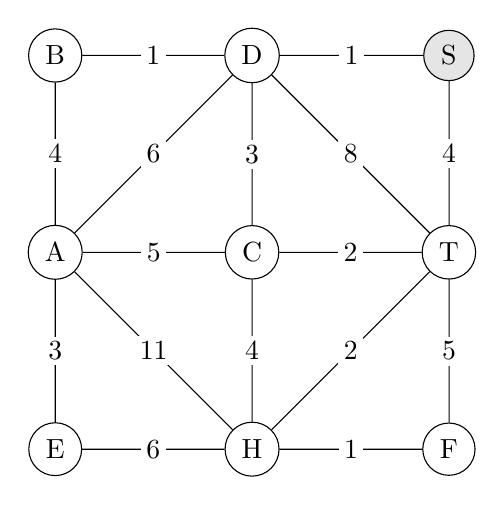
\begin{tikzpicture}[scale=2.5, lbl/.style={midway, fill=white, inner sep = 2pt}]
\node[draw, circle] (A) at (1,0) {A} ;
\node[draw, circle] (B) at (1,1) {B} ;
\node[draw, circle] (C) at (2,0) {C} ;
\node[draw, circle] (D) at (2,1) {D} ;
\node[draw, circle] (T) at (3,0) {T} ;
\node[draw, circle, fill=gray!20] (S) at (3,1) {S} ;
\node[draw, circle] (H) at (2,-1) {H} ;
\node[draw, circle] (F) at (3,-1) {F} ;
\node[draw, circle] (E) at (1,-1) {E};

\draw (A) -- node[lbl]{4}(B)  -- node[lbl]{1} (D) -- node[lbl]{3}(C) -- node[lbl]{2} (T) -- node[lbl]{5}(F);
\draw (A) -- node[lbl] {5} (C)  -- node[lbl] {4}(H)  -- node[lbl] {1} (F);
\draw (S) -- node[lbl] {4} (T) ;
\draw (D) -- node[lbl]{1} (S) ;\draw (H) -- node[lbl]{11} (A);
\draw (T) -- node[lbl]{2}(H) ;\draw (D) -- node[lbl]{6}(A);
\draw (D) -- node[lbl] {8} (T);
\draw (A) -- node[lbl]{3} (E);
\draw (E) -- node[lbl]{6}(H);
\end{tikzpicture}
\end{adjustbox}
%\hfill
\begin{adjustbox}{valign=t,minipage={.25\textwidth}}
\begingroup
\renewcommand{\arraystretch}{1.5}
 \begin{tabular}{ |c | c |c| c|}
 \hline
 &&\textbf{tentative}&\\
 vertex & current/ & minimum& preceding\\ 
 &visited&\quad distance to $E$ \quad& vertex\\
 \hline
A&&& \\
\hline 
B&&& \\
\hline 
C&&& \\
\hline 
D&&& \\
\hline 
E&&& \\
\hline 
F&&& \\
\hline 
H&&& \\
\hline 
S&&& \\
\hline 
T&&& \\
\hline 
 \end{tabular}
\endgroup
\end{adjustbox}


\vspace{1cm}

Length of the shortest path from $S$ to $E$: \underline{\hspace{1in}}\\

Find the shortest path from $S$ to $E$ \emph{using the last column in the table.}
\vfill

\newpage

\item We can also use Dijkstra's algorithm to find the shortest distance between two vertices in a graph that does not have weights on the edges, by assuming all of the weights are 1. Find a shortest path between vertex A and vertex T. As usual, break ties alphabetically.

\begin{adjustbox}{valign=t,minipage={.4\textwidth}}
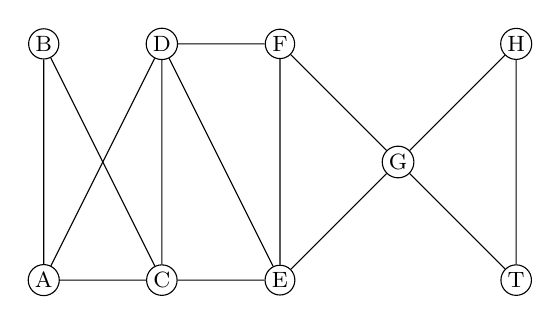
\begin{tikzpicture}[baseline=(current bounding box.center), xscale=.5]
\tikzstyle{every node}=[circle, draw, fill=black!0,
                        inner sep=1pt, minimum width=10pt, font = \footnotesize]
\node (A) at (0,0) {A} ;
\node (B)  at (0,3) {B};
\node (C) at (3,0) {C} ;
\node (E) at (6,0) {E} ;
\node (F) at (6,3)  {F} ;
\node (D) at (3,3)  {D};
\node (G) at (9, 1.5) {G};
\node (H) at (12, 3) {H};
\node (I) at (12, 0) {T};
\draw (A) -- (B) -- (C) -- (D) -- (F);
\draw  (F)--(G) -- (E) -- (F);
\draw (D)-- (E) --(C) --(A)--(D);
\draw (H)--(I)--(G)--(H);
\end{tikzpicture}
%\end{center}
\end{adjustbox}
%
\begin{adjustbox}{valign=t,minipage={.25\textwidth}}

\begingroup
\renewcommand{\arraystretch}{1.5}
 \begin{tabular}{ |c | c |c| c|}
 \hline
 &&\textbf{tentative}&\\
 vertex & current/ & minimum& preceding\\ 
 &visited&\quad distance to $T$ \quad& vertex\\
 \hline
 A&&& \\
\hline 
B&&& \\
\hline 
C&&& \\
\hline 
D&&& \\
\hline 
E&&& \\
\hline 
F&&& \\
\hline 
G&&& \\
\hline 
H&&& \\
\hline 
T&&& \\
\hline 
 \end{tabular}
\endgroup



\end{adjustbox}

\bigskip

Length of the shortest path from $A$ to $T$: \underline{\hspace{1in}}\\

Find the shortest path from $A$ to $T$ \emph{using the last column in the table.}
\vfill

\end{enumerate}

\end{document}

%-------------------------------------------------------------------------------------------------------------------------------------------------------------------------------------------------------------------

%%% Local Variables:
%%% mode: latex
%%% TeX-master: t
%%% End:
